\documentclass{standalone}
\usepackage{tikz}
\usetikzlibrary{patterns, positioning}
\usepackage[sfdefault]{ClearSans} %% option 'sfdefault' activates Clear Sans as the default text font
\usepackage[T1]{fontenc}

\begin{document}
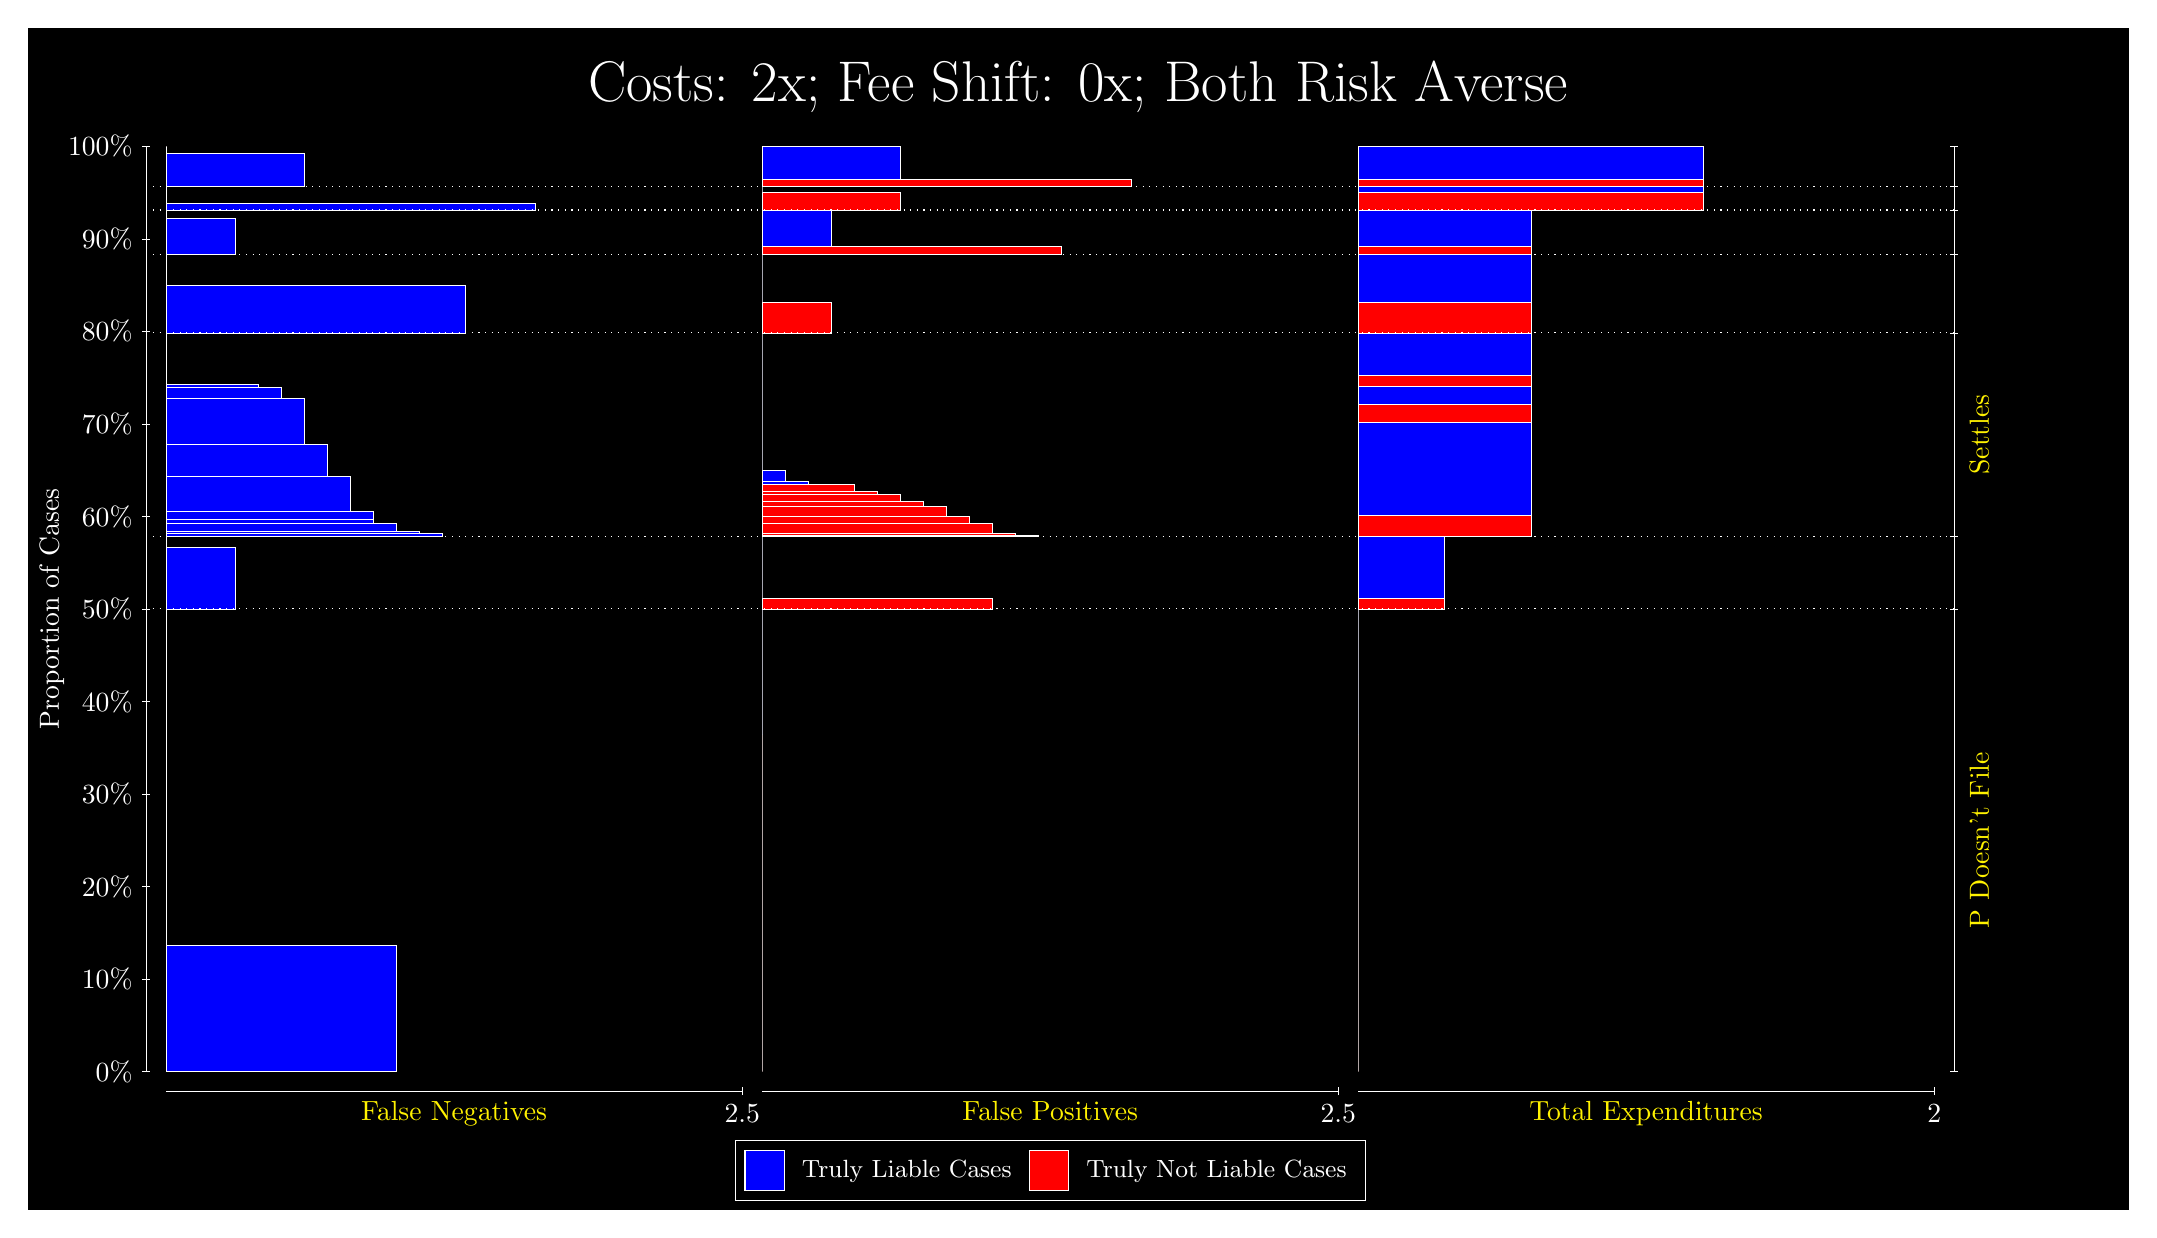
\begin{tikzpicture}
\draw[fill=black] (0,0) rectangle (26.667,15);
\draw[text=white] (0,13.5) rectangle (26.667,15) node[midway] {\huge Costs: 2x; Fee Shift: 0x; Both Risk Averse};
\draw[white, very thin] (1.5,1.75) -- (1.5,13.5);
\node[rotate=90, text=white, anchor=center] at (0.3, 7.625) {Proportion of Cases};
\draw[white, very thin] (1.45,1.75) -- (1.55,1.75);
\node[text=white, anchor=east] at (1.45, 1.75) {0\%};
\draw[white, very thin] (1.45,2.925) -- (1.55,2.925);
\node[text=white, anchor=east] at (1.45, 2.925) {10\%};
\draw[white, very thin] (1.45,4.1) -- (1.55,4.1);
\node[text=white, anchor=east] at (1.45, 4.1) {20\%};
\draw[white, very thin] (1.45,5.275) -- (1.55,5.275);
\node[text=white, anchor=east] at (1.45, 5.275) {30\%};
\draw[white, very thin] (1.45,6.45) -- (1.55,6.45);
\node[text=white, anchor=east] at (1.45, 6.45) {40\%};
\draw[white, very thin] (1.45,7.625) -- (1.55,7.625);
\node[text=white, anchor=east] at (1.45, 7.625) {50\%};
\draw[white, very thin] (1.45,8.8) -- (1.55,8.8);
\node[text=white, anchor=east] at (1.45, 8.8) {60\%};
\draw[white, very thin] (1.45,9.975) -- (1.55,9.975);
\node[text=white, anchor=east] at (1.45, 9.975) {70\%};
\draw[white, very thin] (1.45,11.15) -- (1.55,11.15);
\node[text=white, anchor=east] at (1.45, 11.15) {80\%};
\draw[white, very thin] (1.45,12.325) -- (1.55,12.325);
\node[text=white, anchor=east] at (1.45, 12.325) {90\%};
\draw[white, very thin] (1.45,13.5) -- (1.55,13.5);
\node[text=white, anchor=east] at (1.45, 13.5) {100\%};

\draw[white, very thin] (24.457,1.75) -- (24.457,13.5);
\draw[white, very thin] (24.407,1.75) -- (24.507,1.75);
\node[anchor=west] at (24.407, 1.75) {};
\draw[white, very thin] (24.407,7.6266) -- (24.507,7.6266);
\node[anchor=west] at (24.407, 7.6266) {};
\draw[white, very thin] (24.407,8.5494) -- (24.507,8.5494);
\node[anchor=west] at (24.407, 8.5494) {};
\draw[white, very thin] (24.407,11.131) -- (24.507,11.131);
\node[anchor=west] at (24.407, 11.131) {};
\draw[white, very thin] (24.407,12.127) -- (24.507,12.127);
\node[anchor=west] at (24.407, 12.127) {};
\draw[white, very thin] (24.407,12.691) -- (24.507,12.691);
\node[anchor=west] at (24.407, 12.691) {};
\draw[white, very thin] (24.407,12.995) -- (24.507,12.995);
\node[anchor=west] at (24.407, 12.995) {};
\draw[white, very thin] (24.407,13.5) -- (24.507,13.5);
\node[anchor=west] at (24.407, 13.5) {};

\draw[white, very thin, fill=blue] (1.75,1.75) rectangle (4.6775,3.3497);
\draw[white, very thin, fill=red] (1.75,3.3497) rectangle (1.75,7.6266);
\draw[white, very thin, fill=blue] (1.75,7.6266) rectangle (2.6283,8.4118);
\draw[white, very thin, fill=red] (1.75,8.4118) rectangle (1.75,8.5494);
\draw[white, very thin, fill=blue] (1.75,8.5494) rectangle (5.2631,8.5818);
\draw[white, very thin, fill=blue] (1.75,8.5818) rectangle (4.9703,8.6114);
\draw[white, very thin, fill=blue] (1.75,8.6114) rectangle (4.6775,8.7129);
\draw[white, very thin, fill=blue] (1.75,8.7129) rectangle (4.3848,8.7688);
\draw[white, very thin, fill=blue] (1.75,8.7688) rectangle (4.3848,8.8607);
\draw[white, very thin, fill=blue] (1.75,8.8607) rectangle (4.092,9.3092);
\draw[white, very thin, fill=blue] (1.75,9.3092) rectangle (3.7993,9.7149);
\draw[white, very thin, fill=blue] (1.75,9.7149) rectangle (3.5065,10.298);
\draw[white, very thin, fill=blue] (1.75,10.298) rectangle (3.2138,10.437);
\draw[white, very thin, fill=blue] (1.75,10.437) rectangle (2.921,10.478);
\draw[white, very thin, fill=red] (1.75,10.478) rectangle (1.75,11.131);
\draw[white, very thin, fill=blue] (1.75,11.131) rectangle (5.5558,11.733);
\draw[white, very thin, fill=red] (1.75,11.733) rectangle (1.75,12.127);
\draw[white, very thin, fill=blue] (1.75,12.127) rectangle (2.6283,12.582);
\draw[white, very thin, fill=red] (1.75,12.582) rectangle (1.75,12.691);
\draw[white, very thin, fill=blue] (1.75,12.691) rectangle (6.4341,12.774);
\draw[white, very thin, fill=red] (1.75,12.774) rectangle (1.75,12.995);
\draw[white, very thin, fill=blue] (1.75,12.995) rectangle (3.5065,13.416);
\draw[white, very thin, fill=red] (1.75,13.416) rectangle (1.75,13.5);
\draw[white, very thin, fill=red] (9.3189,1.75) rectangle (9.3189,6.027);
\draw[white, very thin, fill=blue] (9.3189,6.027) rectangle (9.3189,7.6266);
\draw[white, very thin, fill=red] (9.3189,7.6266) rectangle (12.246,7.7643);
\draw[white, very thin, fill=blue] (9.3189,7.7643) rectangle (9.3189,8.5494);
\draw[white, very thin, fill=red] (9.3189,8.5494) rectangle (12.832,8.5609);
\draw[white, very thin, fill=red] (9.3189,8.5609) rectangle (12.539,8.5903);
\draw[white, very thin, fill=red] (9.3189,8.5903) rectangle (12.246,8.7083);
\draw[white, very thin, fill=red] (9.3189,8.7083) rectangle (11.954,8.8011);
\draw[white, very thin, fill=red] (9.3189,8.8011) rectangle (11.661,8.9237);
\draw[white, very thin, fill=red] (9.3189,8.9237) rectangle (11.368,8.9892);
\draw[white, very thin, fill=red] (9.3189,8.9892) rectangle (11.075,9.077);
\draw[white, very thin, fill=red] (9.3189,9.077) rectangle (10.783,9.1218);
\draw[white, very thin, fill=red] (9.3189,9.1218) rectangle (10.49,9.2021);
\draw[white, very thin, fill=blue] (9.3189,9.2021) rectangle (9.9044,9.2433);
\draw[white, very thin, fill=blue] (9.3189,9.2433) rectangle (9.6116,9.3819);
\draw[white, very thin, fill=blue] (9.3189,9.3819) rectangle (9.3189,11.131);
\draw[white, very thin, fill=red] (9.3189,11.131) rectangle (10.197,11.525);
\draw[white, very thin, fill=blue] (9.3189,11.525) rectangle (9.3189,12.127);
\draw[white, very thin, fill=red] (9.3189,12.127) rectangle (13.125,12.235);
\draw[white, very thin, fill=blue] (9.3189,12.235) rectangle (10.197,12.691);
\draw[white, very thin, fill=red] (9.3189,12.691) rectangle (11.075,12.912);
\draw[white, very thin, fill=blue] (9.3189,12.912) rectangle (9.3189,12.995);
\draw[white, very thin, fill=red] (9.3189,12.995) rectangle (14.003,13.079);
\draw[white, very thin, fill=blue] (9.3189,13.079) rectangle (11.075,13.5);
\draw[white, very thin, fill=red] (16.888,1.75) rectangle (16.888,6.027);
\draw[white, very thin, fill=blue] (16.888,6.027) rectangle (16.888,7.6266);
\draw[white, very thin, fill=red] (16.888,7.6266) rectangle (17.986,7.7643);
\draw[white, very thin, fill=blue] (16.888,7.7643) rectangle (17.986,8.5494);
\draw[white, very thin, fill=red] (16.888,8.5494) rectangle (19.083,8.8193);
\draw[white, very thin, fill=blue] (16.888,8.8193) rectangle (19.083,9.9898);
\draw[white, very thin, fill=red] (16.888,9.9898) rectangle (19.083,10.23);
\draw[white, very thin, fill=blue] (16.888,10.23) rectangle (19.083,10.449);
\draw[white, very thin, fill=red] (16.888,10.449) rectangle (19.083,10.592);
\draw[white, very thin, fill=blue] (16.888,10.592) rectangle (19.083,11.131);
\draw[white, very thin, fill=red] (16.888,11.131) rectangle (19.083,11.525);
\draw[white, very thin, fill=blue] (16.888,11.525) rectangle (19.083,12.127);
\draw[white, very thin, fill=red] (16.888,12.127) rectangle (19.083,12.235);
\draw[white, very thin, fill=blue] (16.888,12.235) rectangle (19.083,12.691);
\draw[white, very thin, fill=red] (16.888,12.691) rectangle (21.279,12.912);
\draw[white, very thin, fill=blue] (16.888,12.912) rectangle (21.279,12.995);
\draw[white, very thin, fill=red] (16.888,12.995) rectangle (21.279,13.079);
\draw[white, very thin, fill=blue] (16.888,13.079) rectangle (21.279,13.5);
\draw[white, dotted] (1.5,7.6266) -- (24.457,7.6266);
\draw[white, dotted] (1.5,8.5494) -- (24.457,8.5494);
\draw[white, dotted] (1.5,11.131) -- (24.457,11.131);
\draw[white, dotted] (1.5,12.127) -- (24.457,12.127);
\draw[white, dotted] (1.5,12.691) -- (24.457,12.691);
\draw[white, dotted] (1.5,12.995) -- (24.457,12.995);
\draw[white, very thin] (1.75,1.5) -- (9.0689,1.5);
\node[text=yellow, anchor=north] at (5.4094, 1.5) {False Negatives};
\draw[white, very thin] (9.0689,1.45) -- (9.0689,1.55);
\node[text=white, anchor=north] at (9.0689, 1.45) {2.5};

\draw[white, very thin] (9.3189,1.5) -- (16.638,1.5);
\node[text=yellow, anchor=north] at (12.978, 1.5) {False Positives};
\draw[white, very thin] (16.638,1.45) -- (16.638,1.55);
\node[text=white, anchor=north] at (16.638, 1.45) {2.5};

\draw[white, very thin] (16.888,1.5) -- (24.207,1.5);
\node[text=yellow, anchor=north] at (20.547, 1.5) {Total Expenditures};
\draw[white, very thin] (24.207,1.45) -- (24.207,1.55);
\node[text=white, anchor=north] at (24.207, 1.45) {2};

\node[text=yellow, centered, rotate=90] at (24.777, 4.6883) {P Doesn't File};

\node[text=yellow, centered, rotate=90] at (24.777, 9.8401) {Settles};





\draw (12.978300999999998,1.5) node[draw=none] (baseCoordinate) {};
\begin{scope}[align=center]
        \matrix[scale=0.5, draw=white, below=0.5cm of baseCoordinate, nodes={draw}, column sep=0.1cm]{
            \node[rectangle, draw, minimum width=0.5cm, minimum height=0.5cm, fill=blue] {}; &
            \node[draw=none, font=\small, text=white] (B) {Truly Liable Cases}; &
            \node[rectangle, draw, minimum width=0.5cm, minimum height=0.5cm, fill=red] {}; &
            \node[draw=none, font=\small, text=white] (B) {Truly Not Liable Cases}; \\
            };
\end{scope}

\end{tikzpicture}
\end{document}